\section{Results}
\label{sec:results}

\subsection{Primary study (DeepSeek V4 Pro / hardship-support routing)}

100 pairs, 1{,}300 calls, 100\% provider success, EUR 2.66.

\begin{table}[t]
\setlength{\tabcolsep}{4.5pt}
\caption{Primary study (DeepSeek V4 Pro, hardship-support routing).}
\label{tab:primary}
\begin{tabular}{@{}ll@{}}
\toprule
\textbf{Metric} & \textbf{Value} \\
\midrule
BACC A0 (no purpose) & 0.32 \\
BACC A1 (full purpose) & 0.71 \\
BACC A3 (governed) & 0.71 \\
UIR P0 (prohibited, visible) & 1.00 \\
UIR P2 (masked, deterministic) & 0.00 \\
UIR P3 (masked, contract) & 0.00 \\
ND floor & 0.00 \\
\bottomrule
\end{tabular}

\medskip
\begin{tabular}{@{}llll@{}}
\toprule
\textbf{Hyp.} & \textbf{Decision} & \textbf{Point} & \textbf{$p$ (1-sided)} \\
\midrule
H1 gain & PASS & 0.39 & 0.00020 \\
H2 AUR & PASS & 1.0 & --- \\
H3 NetUI & PASS & 1.00 & 0.00020 \\
H5 suppression & PASS & $-1.00$ & 0.0 \\
H6 P3 vs.\ floor & PASS & $-0.00$ & 0.0 \\
H7 P2 $=$ P3 & EQUIV. & 0.00 & $p_{\mathrm{TOST}}$ 0.0 \\
\bottomrule
\end{tabular}
\end{table}

Table~\ref{tab:primary} summarizes the primary study. Declaring purpose raised
balanced accuracy from 0.32 (no purpose) to 0.71 (H1 gain 0.39, 95\% CI
[0.21, 0.56], $p = 0.00020$); governed execution retained the entire gain
(AUR $= 1.0$, 95\% CI [1.0, 1.0], H2). Prohibited-visible data changed the
decision on \emph{every} pair (UIR$_{P0} = 1.00$ versus a floor of 0.00; H3 net
influence 1.00, 95\% CI [1.00, 1.00], McNemar exact $p = 1.58\times10^{-30}$),
and both masking variants suppressed that influence exactly (UIR $= 0.00$;
H5, H6).

\subsection{Replication study (Kimi K3 / fraud review)}

120 pairs, 1{,}560 calls, 99.0\% provider success.

\begin{table}[t]
\setlength{\tabcolsep}{3.5pt}
\caption{Replication study (Kimi K3, fraud review).}
\label{tab:replication}
\begin{tabular}{@{}ll@{}}
\toprule
\textbf{Metric} & \textbf{Value} \\
\midrule
BACC A0 (no purpose) & 0.625 \\
BACC A1 (full purpose) & 0.7333 \\
BACC A3 (governed) & 0.7333 \\
UIR P0 (prohibited, visible) & 0.9646 \\
UIR P2 (masked, deterministic) & 0.00 \\
UIR P3 (masked, contract) & 0.0083 \\
ND floor & 0.0375 \\
\bottomrule
\end{tabular}

\medskip
\begin{tabular}{@{}llll@{}}
\toprule
\textbf{Hyp.} & \textbf{Decision} & \textbf{Point} & \textbf{$p$ (1-sided)} \\
\midrule
H1 gain & PASS & 0.1083 & 0.00200 \\
H2 AUR & PASS & 1.0 & --- \\
H3 NetUI & PASS & 0.9292 & 0.00020 \\
H5 suppression & PASS & $-0.9646/-0.9558$ & 0.0 \\
H6 P3 vs.\ floor & PASS & $-0.0292$ & 0.0236 \\
H7 P2 $=$ P3 & EQUIV. & $-0.0083$ & $p_{\mathrm{TOST}}$ $9.98\times10^{-7}$ \\
\bottomrule
\end{tabular}
\end{table}

The replication (Table~\ref{tab:replication}) reproduces every gate on a
second model family and a second task. Purpose gain 0.1083 (95\% CI
[0.033, 0.175], $p = 0.00200$); AUR $= 1.0$; prohibited-visible influence
0.9646 against a floor of 0.0375 (net 0.9292, 95\% CI [0.8805, 0.9646],
McNemar $p = 3.94\times10^{-31}$); masking suppressed influence to 0.00 (P2)
and 0.0083 (P3), with P3 statistically equivalent to the floor within the 0.05
margin (H6, point $-0.0292$, 95\% CI $[-0.0625, 0.0]$, $p = 0.0236$) and P2
equivalent to P3 (H7, $p_{\mathrm{TOST}} = 9.98\times10^{-7}$).

\begin{figure}[t]
  \centering
  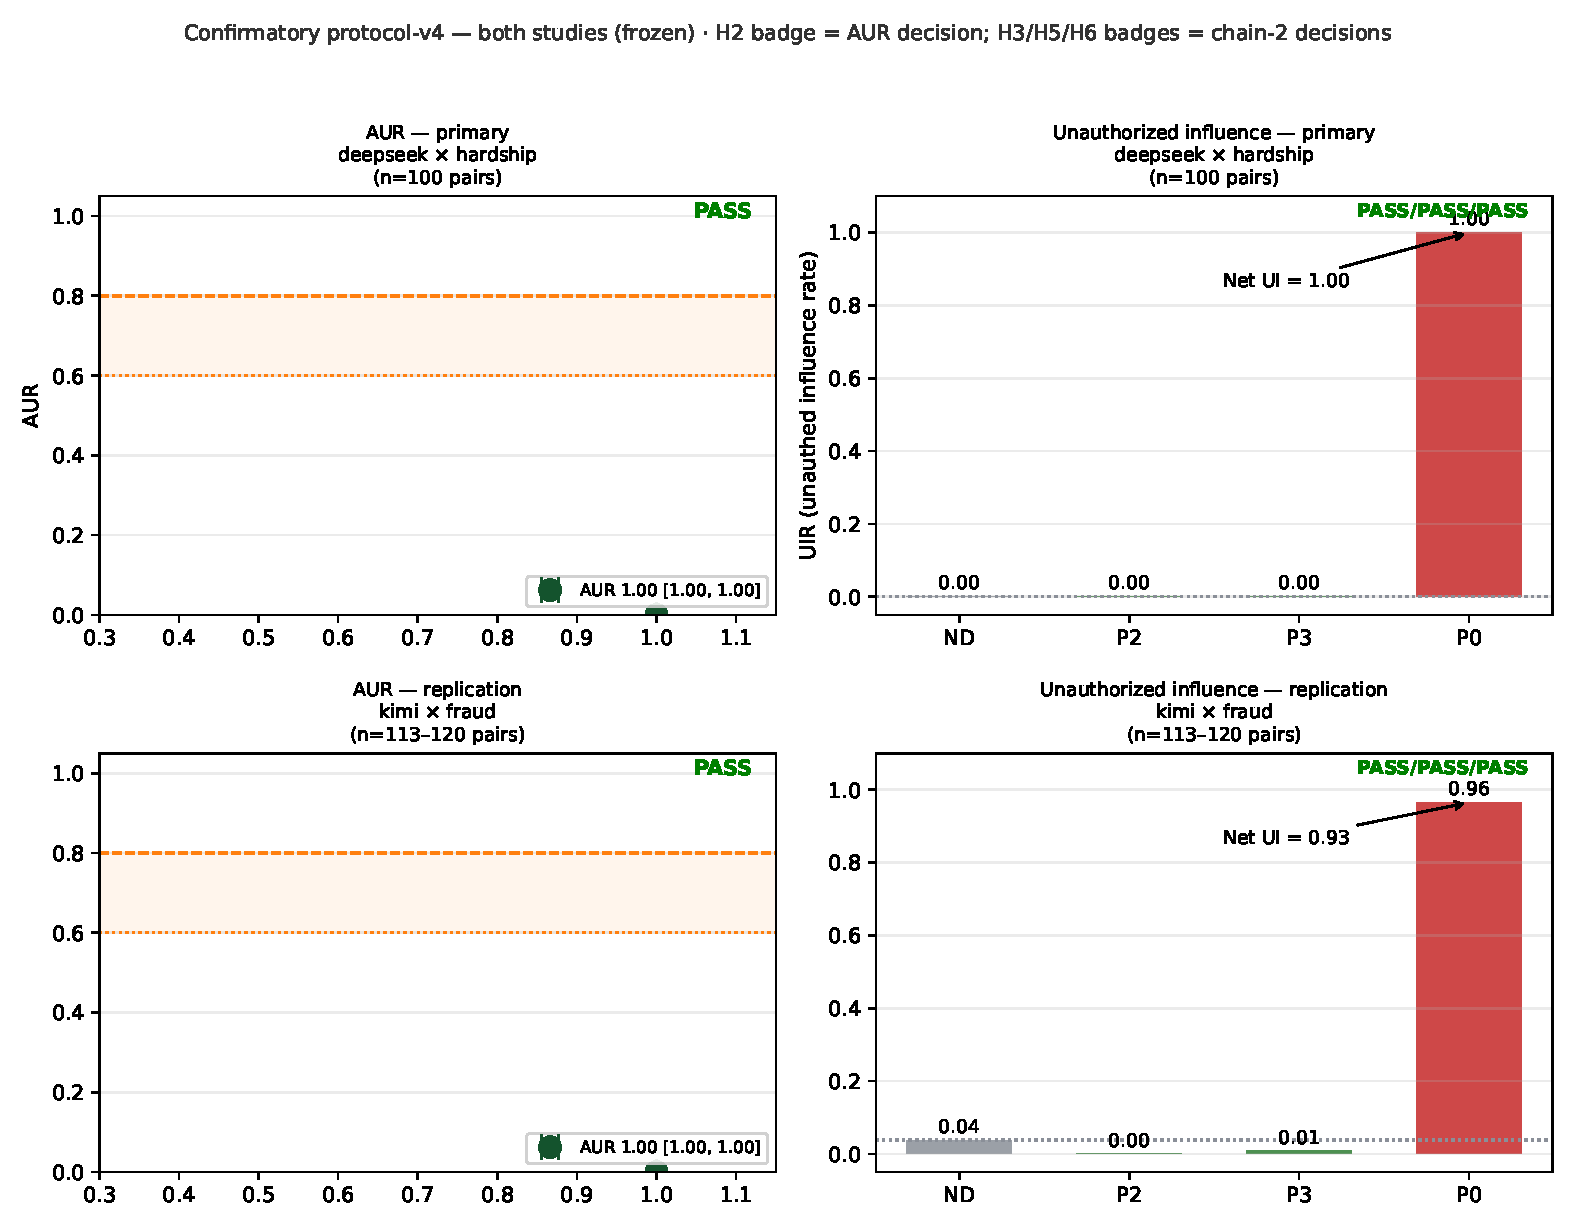
\includegraphics[width=\columnwidth]{generated/headline-figure.pdf}
  \caption{Headline results. Rows: primary study (top), replication study
  (bottom). Left panels: authorized utility (BACC) per condition, with the
  governed condition (A3) equal to the full-purpose condition (A1).
  Right panels: unjustified influence rate (UIR) per condition against the
  natural-decision floor; prohibited-visible data (P0) sits at or near 1.0
  while masked variants (P2, P3) sit at or below the floor.}
  \label{fig:headline}
\end{figure}

\subsection{Combined interpretation}

Both studies passed every pre-registered gate, satisfying interpretation rule
1: \emph{the effect reproduces across two model families and two financial
tasks}. The frozen evidence was re-computed independently (fresh
implementation over raw events, no shared code with the reporting scripts):
17/17 verification checks pass, including exact reproduction of every headline
metric in Tables~\ref{tab:primary} and~\ref{tab:replication} and both McNemar
$p$-values.

\subsection{What the results do and do not show}

The governed condition (A3) and the masked conditions (P2, P3) were equivalent
in influence in both studies, and governed execution retained the full
authorized gain. We make no claim that governed execution \emph{outperforms}
masking: on a single narrow field, deterministic masking (P2) and contract
masking (P3) are behaviorally indistinguishable, as the H7 equivalence shows.
The contribution is that the \emph{same} adapter that improves authorized
accuracy by carrying purpose context (A1 $\to$ A3) also enforces the prohibited
boundary (P3) at the floor, jointly satisfying Equation~\eqref{eq:psbe} in
every condition tested.
